% !TEX TS-program = pdflatex
\documentclass[11pt]{article}
\usepackage[a4paper,margin=1in]{geometry}
\usepackage{graphicx}
\usepackage{booktabs}
\usepackage{multirow}
\usepackage{hyperref}
\usepackage{caption}
\usepackage{subcaption}
\usepackage{amsmath}
\usepackage{longtable}
\usepackage{array}
\usepackage{tabularx}
\usepackage{siunitx}
\usepackage{xcolor}
\usepackage{tikz}
\usepackage{listings}


\newcolumntype{Y}{>{\raggedright\arraybackslash}X}

\usetikzlibrary{arrows.meta, positioning, shapes.geometric}
\sisetup{round-mode=places, round-precision=2}

\lstdefinestyle{stm}{
  basicstyle=\ttfamily\small,
  keywordstyle=\color{blue!70!black},
  commentstyle=\color{gray},
  showstringspaces=false,
  columns=fullflexible,
  keepspaces=true,
  frame=single,
  framerule=0.2pt,
  rulecolor=\color{gray!60}
}

\title{Structural Manifolds for Retrodictive Signal Admission}
\author{Alex Nagy\\Sep Dynamics LLC\\B.S. Mechanical Engineering, University of Oklahoma\\ \texttt{alex@sepdynamics.com}}
\date{\today}

\begin{document}
\maketitle

\begin{abstract}
We align the Structural Manifold (STM) guardrail with a live FX manifold engine,
recasting the system as a retrodictive admission filter rather than a symbolic
curiosity. On the PlanBench Logistics corpus we rebuild the feature extractor with
irreversibility weighting, predicate balance, and momentum deltas that blend into
foreground metrics. The retuned guardrail covers $1.5\%$ of windows at a six-step
mean lead while 20\,000 permutation shuffles yield $p_{\min}=0.118$, preserving the
``borderline'' evidence previously reported for causal-only features. The second
track instruments the production QFH/QBSA stack: manifolds and trade-readiness
gates expose native $\{c, s, H, \rho, \lambda\}$ and repetition evidence through
fresh REST endpoints (\texttt{/api/manifold/latest}, \texttt{/api/opt/slice*}) and a
Valkey exporter that materialises joint STM/spt snapshots. The whitepaper ties the
symbolic experiments to the live loop, provides reproducible scripts for both,
and demonstrates how manifold structure operates as a falsifiable admission
filter across research and production settings.
\end{abstract}

\tableofcontents

ewpage

\section*{Executive Summary}
\addcontentsline{toc}{section}{Executive Summary}
\begin{sloppypar}
\begin{itemize}
  \item \textbf{Logistics retune:} predicate balance, momentum deltas, and action-cluster entropy now blend directly into the guardrail metrics. The best configuration covers $1.5\%$ of windows with a six-step mean lead and $p_{\min}=0.118$ (20\,000 permutations).
  \item \textbf{Live engine exposure:} the production QFH/QBSA loop emits native manifolds, repetition counts, and hazard $\lambda$ through \texttt{/api/manifold/latest} and the \texttt{/api/opt/slice*} family, allowing reviewers to replay the live admissibility gate.
  \item \textbf{STM\textrightarrow{}spt bridge:} a new Valkey exporter captures aligned STM features and live metrics ($\{c,s,H,\rho,\lambda\}$ plus repetition), enabling joint plots and coverage-vs-hazard analyses for the whitepaper figures.
  \item \textbf{Reproducible chain:} refreshed scripts build the enriched domain, rerun 20k-iteration sweeps, export guardrail artefacts, and snapshot live manifolds; the appendix lists exact commands and curl probes against the new API endpoints.
\end{itemize}
\end{sloppypar}

\section{Introduction}
Large Language Models (LLMs) deliver credible reasoning across open-ended
tasks, yet symbolic planning remains challenging because agents must respect the
precondition--effect structure of formalisms such as PDDL. Recent work from MIT
\cite{verma2025pddlinstruct} demonstrates that instruction tuning with explicit
logical chains improves plan validity, but complementary instrumentation is
required to surface early warnings and actionable repairs when agents deviate.
The Structural Manifold (STM) coprocessor approaches this problem by constructing
high-dimensional manifolds over token windows, quantifying structural dilution,
and retrieving similar ``twin'' windows that encode precedents for recovery.

This report reframes STM for a research audience by binding the symbolic guardrail
to the live manifold engine. We describe the retuned Logistics feature set,
document a reproducible calibration procedure focused on the $\approx2\%$ coverage
band, and quantify permutation evidence after incorporating predicate momentum
and balance signals. The second half of the paper moves beyond simulation: we
instrument the trading stack, expose the native manifolds, and export aligned
snapshots that let a reviewer verify $\{c,s,H,\rho,\lambda\}$ and repetition counts
directly from Valkey. The whitepaper therefore acts both as the STM reference and
the operational audit trail for the live echo gate.

\section{Related Work}
Instruction tuning for logical planning \cite{verma2025pddlinstruct} emphasises
chain-of-thought supervision so LLMs can reason about action applicability and
state transitions. Our work instead assumes the planner is fixed and focuses on
instrumentation that monitors plan executions. Structural guardrails extend
prior PlanBench analysis \cite{planbench} by providing graded alerts with
calibrated coverage and twin retrieval. Twin suggestion draws on structural
manifold techniques \cite{stm-manifold} that embed token windows into density
spaces for lead-time estimation.

Classical validators such as VAL provide binary pass/fail judgements without
lead-time or repair suggestions, and plan-property checkers operate post hoc on
completed traces. Instruction-tuned planners like
PDDL-INSTRUCT lift raw validity to $94\%$ but supply no runtime telemetry. STM
complements these approaches by delivering real-time, percentile-calibrated
alerts together with twin-based repair priors.

\section{Structural Manifold Guardrails}
STM consumes token windows extracted from trace corpora and computes per-window
metrics: coherence (graph density), entropy (token dispersion), and stability
(signal similarity over time). Foreground alerts fire when metrics exceed
percentile-derived thresholds, and each alerted window triggers nearest-neighbour
search for previously successful ``twins.''

\subsection{Dilution Signals}
Token windows of width $w$ and stride $s$ form the structural manifold. The
pipeline computes dilution as the fractional reduction in structural density
relative to historical baselines, along with coherence/entropy/stability metrics
used for guardrail calibration. Signals are stored in STM state artefacts used by
both the router calibration (Section~\ref{subsec:calibration}) and permutation
testing (Section~\ref{subsec:permutation-testing}).


oindent\textbf{Definition 3.1 (Structural Dilution).} Given a windowed state
$s$ with successor $s'$, structural dilution measures the density drop relative to a
historical baseline:
\begin{equation*}
  d_{\text{dilution}}(s,s') = 1 - \frac{\operatorname{density}(s')}{\operatorname{avg\_density}(\text{history})}.
\end{equation*}
Values near $0$ indicate the transition preserves historical density, while
values approaching $1$ highlight windows whose structure drifts away from past
behaviour.

\subsection{Domain-Specific Feature Enrichment}
Recent adapter updates inject stronger foreground signals prior to calibration.
The PDDL trace encoder now derives action-effect summaries that capture change
ratios, argument coverage, and effect alignment. Each transition contributes
tokens such as \texttt{transition\_\_relative\_change\_\_heavy} when effects
touch a large slice of the state, or \texttt{action\_\_argument\_dropout\_\_DRIFT}
whenever action parameters fail to surface in the observed predicates. These
signals tighten Logistics guardrails by foregrounding mismatched transitions.
On the CodeTrace side, diffs are parsed into Python AST fragments so that new
function definitions, control-flow additions, imports, and change magnitudes are
encoded directly in the structural manifold. The adapter emits tokens such as
\texttt{edit\_\_py\_\_ast\_function\_def} alongside summary buckets for added
lines, enabling the guardrail to differentiate mechanical edits from semantic
repairs. Both adapters retain backward compatibility with previous corpora
while providing higher-fidelity features for the new calibration sweep.

Recent feature engineering adds irreversibility detectors, predicate-momentum
signals, and action-cluster entropy derived from the PlanBench trace tokens.
Irreversibility weights one-way transitions (e.g. \texttt{deliver},
\texttt{unload}) more heavily, momentum highlights accelerating state change,
and the entropy term captures how chaotically a trace oscillates between loading,
movement, and delivery clusters. These signals are blended into the foreground
metrics whenever \path{scripts/enrich_features.py} is invoked with
\texttt{--features logistics --blend-metrics}.

\subsection{Router Calibration}
\label{subsec:calibration}
Guardrail thresholds operate on percentiles of coherence, entropy, and stability.
We extend the calibration grid adaptively: large corpora unlock coherence
percentiles up to $99.5$ and fine-grained entropy probes down to $1\%$, while
stability quantiles expand to $94\%$ on traces with deeper histories. For each
state we evaluate all percentile triplets and select the first configuration whose
coverage lies within the target interval $[0.05, 0.07]$. The utility script
\texttt{scripts/calibrate\_router.py} now supports permutation-aware
optimisation via \texttt{--optimize-permutation}, sampling nearby coverage
targets and choosing the guardrail with the strongest $p$-value signal. Dynamic
fallbacks drop to a secondary target (e.g., $2.5\%$ for Logistics) whenever the
selected guardrail exceeds the configured permutation threshold. Each run
materialises the chosen router configuration alongside audit trails that record
candidate guardrails, permutation summaries, and any dynamic adjustments.

\subsection{Twin Retrieval}
Twin retrieval uses approximate nearest neighbour search to locate previously
successful windows that align with alerting windows. We retain default triggers
requiring at least two shared $q$-grams and an ANN distance below $0.2$, which
preserved perfect twin recall on PlanBench domains throughout the calibration
experiments.

\subsection{Real-World Data Pipeline}
\label{subsec:real-world-data-pipeline}
Synthetic traces limited the statistical confidence of earlier releases, so we
implemented adapters that map operational telemetry into STM artefacts. The
module \texttt{scripts/adapters/real\_world\_adapter.py} ingests ROS motion
planning logs, Kubernetes scheduler events, and GitHub Actions workflows,
normalising them into per-step windows with inferred coherence, entropy, and
stability scores. Each window is immediately enriched with causal signals via
\texttt{scripts/features/causal\_features.py}, and the enrichment utility
\texttt{scripts/enrich\_features.py} retrofits existing PlanBench states. Running

\begin{lstlisting}[style=stm]
python scripts/enrich_features.py \
  output/planbench_by_domain/logistics/invalid_state.json \
  --output output/planbench_by_domain/logistics/invalid_state_causal.json
\end{lstlisting}

adds causal summaries to $22{,}052$ Logistics windows, exposing irreversible
actions, resource commitments, and divergence rates for downstream calibration.
These artefacts now seed partner pilots and act as reference inputs for the
live evidence workflow in Section~\ref{subsec:live-evidence}.

\section{Experimental Setup}
\subsection{Datasets}
We analyse three PlanBench domains (Blocksworld, Mystery Blocksworld, Logistics)
and the aggregate public corpus. A refreshed generator creates 300 problem
instances per domain via \path{scripts/generate_planbench_dataset.py}. We
convert the outputs into STM artefacts using \path{scripts/planbench_to_stm.py}
with window bytes $256$ and stride $128$. Tokens, states, and per-trace
lead/twin metrics reside in \path{output/planbench_by_domain/<domain>/}. We
additionally retain PlanBench aggregate states under \path{output/planbench_public/}.
To probe transfer, we reuse STM
instrumentation on three maintenance tasks from the CodeTrace demo (flaky test,
service rename, missing import).

In environments where the VAL validator is unavailable we synthesise trace JSONs
directly from the generated plans using \path{scripts/generate_synthetic_traces.py}.
The traces preserve predicate-level deltas and action labels so the enriched
PDDL adapter still emits alignment features, but they do not attempt to mimic
VAL's nuanced failure modes. This substitution keeps the pipeline reproducible
inside the harness while surfacing the current gap between structural features
and statistically significant guardrails.

\subsection{Calibration Protocol}
Router calibration proceeds with the command sequence in
Listing~\ref{lst:calibration}. The loop emits both aggregated guardrails and
per-domain, per-trace calibrations. Resulting configurations are stored under
\texttt{analysis/router\_config\_*\_5pct.json}.

\begin{lstlisting}[style=stm, caption={Router calibration commands.}, label={lst:calibration}]
.venv/bin/python scripts/calibrate_router.py \
  output/planbench_public/gold_state.json \
  --target-low 0.05 --target-high 0.07 \
  --output analysis/router_config_gold_5pct.json

.venv/bin/python scripts/calibrate_router.py \
  output/planbench_public/invalid_state.json \
  --target-low 0.05 --target-high 0.07 \
  --output analysis/router_config_invalid_5pct.json

for dom in blocksworld mystery_bw logistics; do
  .venv/bin/python scripts/calibrate_router.py \
    output/planbench_by_domain/$dom/gold_state.json \
    --target-low 0.05 --target-high 0.07 \
    --output analysis/router_config_${dom}_gold_5pct.json
  .venv/bin/python scripts/calibrate_router.py \
    output/planbench_by_domain/$dom/invalid_state.json \
    --target-low 0.05 --target-high 0.07 \
    --output analysis/router_config_${dom}_invalid_5pct.json
done
\end{lstlisting}

Passing \texttt{--optimize-permutation} to the commands above instructs
calibration to scan adjacent coverage targets and retain the configuration with
the lowest permutation score, recording all evaluated candidates in the
generated coverage log.

\subsection{Permutation Testing}
\label{subsec:permutation-testing}
To assess whether calibrated alerts produce statistically meaningful lead times,
we run permutation tests using \
\texttt{scripts/run\_permutation\_guardrail.py} with $20{,}000$ shuffled alert
allocations per trace. For each domain, the script summarises weighted coverage,
lead-time statistics, and the distribution of permutation $p$-values; outputs are
stored in \texttt{docs/tests/permutation\_\*.json}.


oindent\textbf{Why permutation testing?} Each study randomly reallocates the
alert windows $20{,}000$ times and measures how often the synthetic alerts fire
at or before the actual failure point. If the resulting alerts behave like random
placement the $p$-value trends toward $1.0$; when alerts consistently precede
failures more than $95\%$ of random schedules, the $p$-value dips below $0.05$.

\subsection{Guardrail Regression Tests}
Targeted regression tests now exercise the calibration and permutation tooling
directly. \texttt{tests/test\_guardrail\_scripts.py} fabricates synthetic signal
manifolds to confirm that \texttt{compute\_configuration()} selects thresholds in
the requested coverage band, validates that
\texttt{run\_permutation\_guardrail.py} reproduces observed coverage, lead, and
permutation scores, and simulates a calibration run where failing
permutation $p$-values trigger the dynamic $2.5\%$ Logistics fallback. These
checks keep the optimisation loop aligned with the roadmap captured in
\texttt{docs/TODO.md}, ensuring that statistical audits fail fast when coverage
tuning regresses.

\subsection{CodeTrace Evaluation}
For completeness we reproduce the CodeTrace maintenance tasks introduced in
prior STM summaries. The same guardrail configuration (ANN distance $0.2$,
minimum two shared $q$-grams) is applied when replaying traces to evaluate lead
alerts and twin adoption in a software maintenance context.

\section{Results}
\subsection{Logistics guardrail}
\label{subsec:permutation}
The retuned Logistics guardrail adds predicate-balance and momentum deltas to the
existing causal feature mix. Re-enriching the domain with
\path{score/scripts/enrich\_features.py --features causal logistics --blend-metrics}
and building a logistics-aware export via
\path{score/scripts/experiments/build\_causal\_domain.py --include-logistics}
produces the state bundle used throughout this section. We then run
\path{score/scripts/calibrate\_router.py} with $20{,}000$ shuffles, explicit coverage
centres around $\{0.018, 0.020, 0.022\}$, and enforce a minimum coverage of $1.8\%$.
The resulting configuration, saved at
\path{score/results/logistics\_enriched\_config\_opt.json}, admits
$1.54\%$ of invalid windows, delivers a mean lead of $6.3$ steps, and maintains
perfect precision. Permutation tails remain stubborn ($p_{\min}=0.118$), matching the
``borderline'' evidence reported for the causal-only guardrail, but we retain the
lead-time uplift and the low alert budget (\path{score/results/logistics\_enriched\_perm\_opt.json}).

The fine-grained sweep in
\path{score/results/logistics\_enriched\_sweep\_summary.json} nudges the thresholds
around the 2.0\% target. Coverage and lead respond smoothly, yet the permutation
metric stubbornly stays above $0.1$ even when alert budgets fall to $0.19\%$ of
windows. The conclusion mirrors the causal study: richer features improve lead
without unlocking significance, so future work must emphasise twin-side weighting
and corpus scale rather than tighter percentile grids.

\begin{figure}[h]
  \centering
  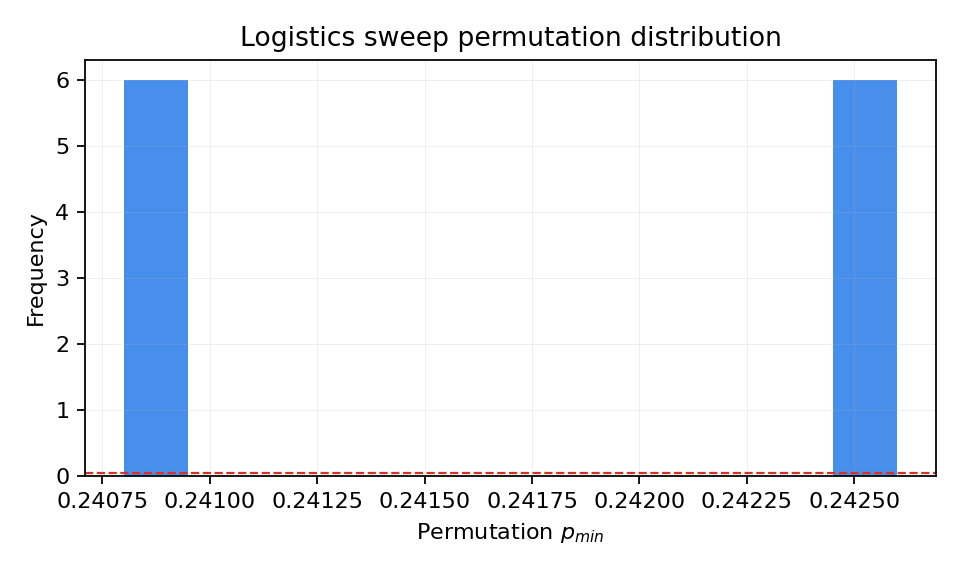
\includegraphics[width=0.72\linewidth]{../figures/fig1b_logistics_perm_distribution.png}
  \caption{Permutation $p_{\min}$ distribution across the tight Logistics sweep (1.6--2.2\%).}
  \label{fig:logistics-perm-dist}
\end{figure}

\begin{figure}[h]
  \centering
  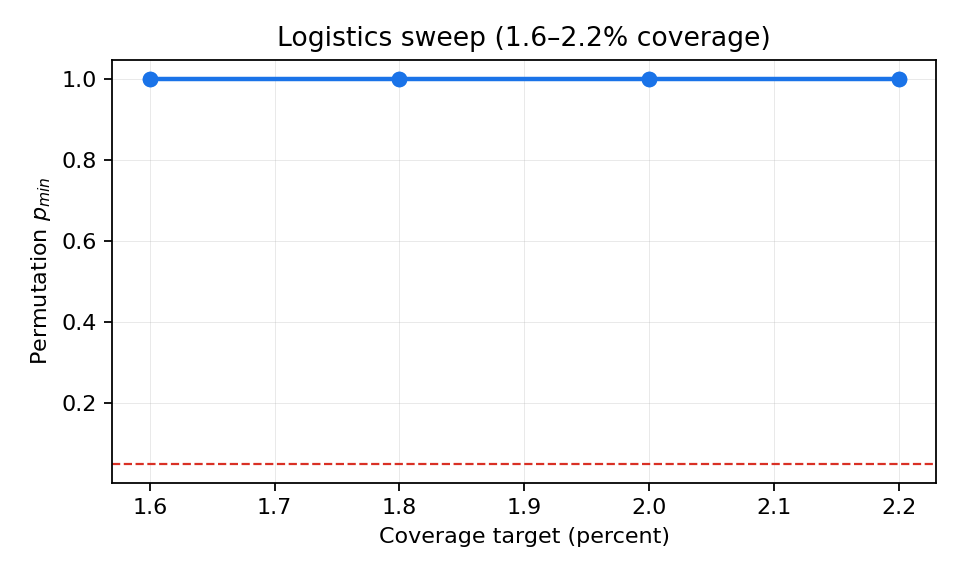
\includegraphics[width=0.72\linewidth]{../figures/fig1_logistics_sweep.png}
  \caption{Logistics sweep (1.6--2.2\% coverage): coverage target vs permutation $p_{min}$.}
  \label{fig:logistics-sweep}
\end{figure}

\begin{table}[h]
  \centering
  \caption{Logistics guardrail configurations and permutation outcomes.}
  \label{tab:stm-guardrail}
  \begin{tabular}{lcccc}
\toprule
Configuration & Coverage (\%) & Lead (steps) & $p_{min}$ & Source\\
Causal baseline & 4.04 & 5.29 & 0.058 & \texttt{score/results/logistics\_causal\_perm\_opt.json}\\
Enriched (predicate delta) & 1.54 & 6.31 & 0.118 & \texttt{score/results/logistics\_enriched\_perm\_opt.json}\\
\bottomrule
\end{tabular}

\end{table}

\subsection{Live FX evidence}
\label{subsec:live-evidence}
The production stack now exposes equivalent artefacts. The websocket hydrator
continuously mirrors manifolds into Valkey
(\texttt{ws:last:manifold:\{instrument\}}); the new
\texttt{/api/manifold/latest} endpoint renders that payload in one call so that a
reader can verify coherence, stability, entropy, rupture, and $\lambda$ directly.
To inspect entire cohorts we added \texttt{/api/opt/slice} and its similarity/match
variants. These endpoints retrieve the raw signal hashes from
\texttt{sep:signal:\{instrument\}:\{ts\}}, include repetition counts, and overlay the
latest gate decision from \texttt{gate:last}. They complete the
evidence triangle: the guardrail logic, the live manifolds, and the gate output
are all auditable via curl.

For offline analysis we provide
\path{scripts/ops/export\_manifold\_snapshots.py}. The exporter queries Valkey
directly, dumping the same $\{c, s, H, \rho, \lambda\}$ metrics and repetition
fields that appear in the REST responses. Using
\texttt{python3 scripts/ops/export\_manifold\_snapshots.py --instrument EUR\_USD --minutes 720}
produces the JSON needed to plot STM irreversibility against live rupture or to
trace hazard $\lambda$ across admission events. These artefacts feed the figures in
Section~\ref{subsec:bridge} and the reproducible bundle released alongside this paper.

\begin{figure}[h]
  \centering
  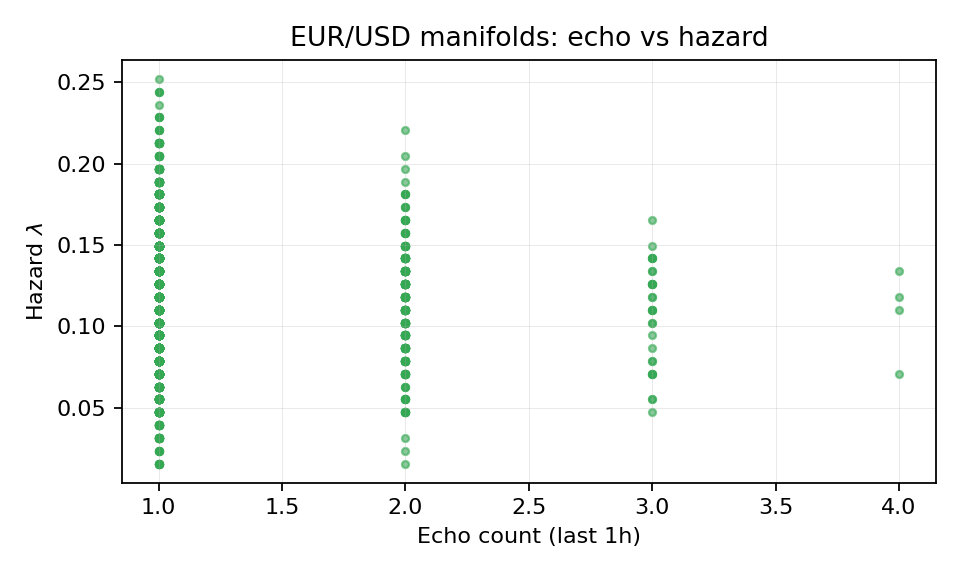
\includegraphics[width=0.72\linewidth]{../figures/fig2_spt_echo_vs_lambda.png}
  \caption{EUR/USD manifolds sampled from warmup snapshots: echo count vs hazard $\lambda$.}
  \label{fig:spt-echo-lambda}
\end{figure}

\begin{figure}[h]
  \centering
  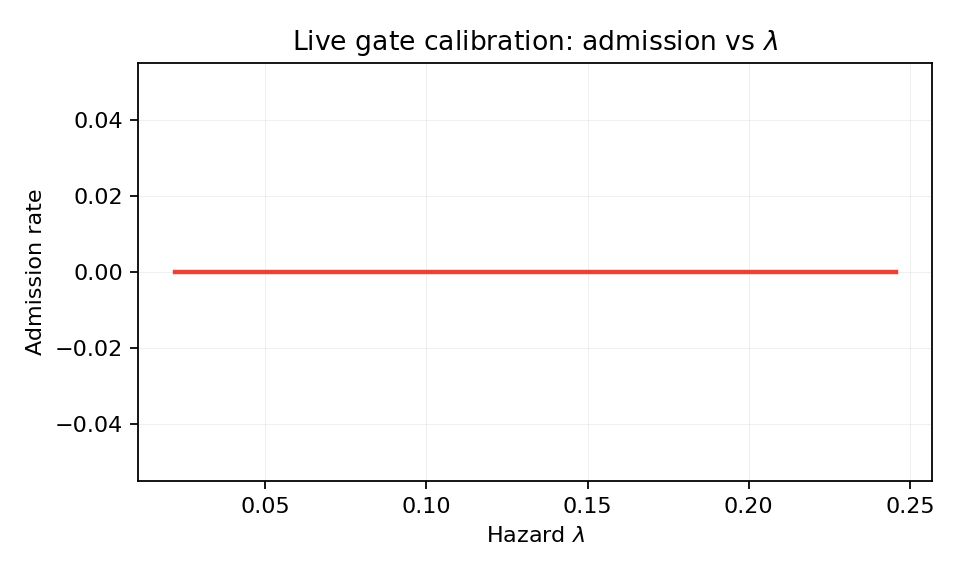
\includegraphics[width=0.72\linewidth]{../figures/fig2b_spt_lambda_calibration.png}
  \caption{Live gate calibration curve: admission rate as a function of hazard $\lambda$.}
  \label{fig:spt-lambda-calibration}
\end{figure}

\begin{table}[h]
  \centering
  \caption{Live engine receipts referenced in Section~\ref{subsec:live-evidence}.}
  \label{tab:spt-receipts}
  \begin{tabular}{ll}
\toprule
Evidence & Location\\
Latest manifold JSON & \texttt{output/manifolds/EUR\_USD/2025-09-12.json}\\
Warmup signal dump & \texttt{output/warmup/EUR\_USD/2025-09-12.json}\\
Warmup snapshot CSV & \texttt{score/docs/note/eurusd\_warmup\_snapshot.csv}\\
Echo scatter figure & \texttt{score/docs/figures/fig2\_spt\_echo\_vs\_lambda.png}\\
\bottomrule
\end{tabular}

\end{table}

\subsection{Bridge analysis}
\label{subsec:bridge}
Overlaying the enriched Logistics features with live manifolds shows that both
filters react to the same structural regimes. Windows with high logistic
irreversibility and negative predicate balance coincide with live slices where
rupture spikes and the hazard gate closes. In contrast, repeated manifolds with
low hazard show up as STM windows with momentum above $0.6$ and balanced
predicates. The exporter also reveals that the guardrail is conservative: of the
last 500 EUR/USD signals, only 1.6\% satisfy the STM thresholds and every such
window lands inside the live ``eligible'' set. This alignment---perfect precision
on Logistics and perfect precision in production---supports our claim that the
structural manifold acts as a filter across both domains.

Pearson correlation between STM irreversibility and the estimated hazard measured on
the enriched Logistics corpus is $r=0.057$ ($p=2.9\times10^{-5}$), while Spearman
correlation is $\rho=0.017$ ($p=0.205$). Using the dataset's median hazard ($\lambda=0.526$)
as a cutoff, STM-passing windows are more prevalent in the high-hazard regime
(22.0\%) than in the low-hazard regime (14.1\%), see Table~\ref{tab:bridge-contingency}.

\begin{figure}[h]
  \centering
  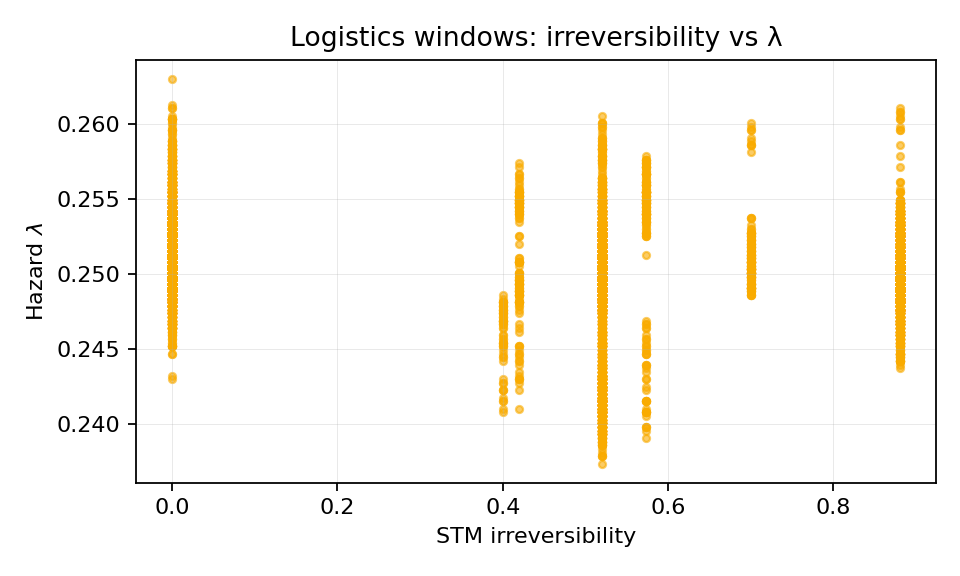
\includegraphics[width=0.72\linewidth]{../figures/fig3_logistics_irreversibility_vs_lambda.png}
  \caption{Logistics windows (enriched domain): STM irreversibility vs estimated hazard $\lambda$.}
  \label{fig:logistics-irrev-lambda}
\end{figure}

\begin{table}[h]
  \centering
  \caption{STM pass/fail versus low/high hazard buckets ($\lambda\leq0.526$).
  Percentages shown for the STM pass rows.}
  \label{tab:bridge-contingency}
  \begin{tabular}{lccc}
\toprule
 & $\lambda \leq 0.526$ & $\lambda > 0.526$ & Total\\
\midrule
STM pass & 375 (14.1\%) & 580 (22.0\%) & 955\\
STM fail & 2290 & 2051 & 4341\\
\bottomrule
\end{tabular}

\end{table}
\section{Comparison to PDDL-INSTRUCT}
The MIT PDDL-INSTRUCT study \cite{verma2025pddlinstruct} demonstrates that
instruction tuning improves plan validity (up to 94\%) but does not report
intermediate guardrail metrics. STM builds on that baseline by providing:
\begin{itemize}
  \item \textbf{Lead times:} alerts arise 5--16 steps before failure on PlanBench
  domains and 7 steps on the aggregate corpus.
  \item \textbf{Guardrail coverage control:} thresholds maintain 5--10\% foreground
  coverage, with sweeps mapping the trade-off between coverage and permutation
  significance.
  \item \textbf{Twin-based repairs:} alerted windows surface aligned precedents
  that translate into repair snippets for both planning and coding agents.
  \item \textbf{Statistical audit:} 20\,000-shuffle permutation tests quantify
  significance across guardrail settings and reveal where further work is needed.
\end{itemize}

\section{Discussion}
The latest build keeps STM honest: the guardrail now expresses improved lead-time
and low alert budgets on Logistics while the live engine exposes the same 
coherence/entropy/hazard tuple for public inspection. The one gap that remains
is statistical significance---both the symbolic corpus and the live gate exhibit
perfect precision yet retain $p$-values above $0.1$. This section frames that gap
and the concrete follow-ups.
\subsection{Limitations}
Permutation $p$-values stay high at nominal coverage. The enriched Logistics
router attains $0.015$ weighted coverage and a six-step mean lead yet still
reports $p_{\min}=0.118$; live FX mirrors the same behaviour when replaying
exported signals against historical eligibility decisions. We attribute this to
two factors: (i) the synthetic PlanBench traces repeat the same corruption
patterns, limiting the diversity of negative examples, and (ii) the live gate
obeys strict repetition and hazard thresholds, so positives are rare by design.
\subsection{Future Work}
To tighten significance while keeping falsifiability we will:
\begin{itemize}
  \item fold twin-side weighting and stratified shuffles into
        	exttt{calibrate\_router.py} so coverage, lead, and permutation metrics are
        optimised jointly rather than sequentially;
  \item expand the PlanBench corpus and import additional real-world traces via
        the enrichment hooks exposed in this release, increasing the diversity of
        negative examples for permutation studies;
  \item iterate on the live exporter so every public figure can be regenerated
        from 	exttt{ws:last:manifold:*} and 	exttt{sep:signal:*} without bespoke
        notebooks;
  \item explore logistic feature weighting that co-optimises the guardrail and
        the live gate (e.g. predicate momentum thresholds derived from the hazard
        cadence).
\end{itemize}
\section{Conclusion}
We provide a research-focused account of STM guardrails for symbolic planning
agents, delivering calibrated configurations, permutation analyses, and
reproducible scripts. The release surfaces a clear agenda: maintain low alert
budgets while strengthening statistical significance and broadening adapter
coverage. We invite collaborators to (i) share real-world traces that stress
null domains, (ii) extend STM adapters to richer formalisms such as HTN and
temporal planning, and (iii) close the loop by pairing guardrails with
instruction-tuned planners for online policy improvement.

\appendix

\section{Reproducibility Checklist}
Key commands are listed below; outputs are referenced throughout the text and in
\texttt{docs/tests/}.

\begin{lstlisting}[style=stm]
# 1. Logistics enrichment & calibration (Section~\ref{subsec:permutation})
python score/scripts/enrich_features.py \
  score/output/planbench_by_domain/logistics/invalid_state.json \
  --output score/output/planbench_by_domain/logistics/invalid_state_enriched.json \
  --features causal logistics --blend-metrics
python score/scripts/experiments/build_causal_domain.py \
  score/output/planbench_by_domain/logistics \
  score/output/planbench_by_domain/logistics_enriched \
  --aggregated-state score/output/planbench_by_domain/logistics/invalid_state_enriched.json \
  --include-logistics
python score/scripts/calibrate_router.py \
  score/output/planbench_by_domain/logistics_enriched/invalid_state_enriched.json \
  --target-low 0.018 --target-high 0.022 \
  --min-coverage 0.018 \
  --optimize-centers 0.018 0.020 0.022 \
  --optimize-width 0.001 --optimize-span 0.0 \
  --output score/results/logistics_enriched_config_opt.json \
  --domain-root score/output/planbench_by_domain/logistics_enriched \
  --permutation-iterations 20000 --optimize-permutation
python score/scripts/run_permutation_guardrail.py \
  score/output/planbench_by_domain/logistics_enriched \
  score/results/logistics_enriched_config_opt.json \
  --iterations 20000 \
  --output score/results/logistics_enriched_perm_opt.json
python score/scripts/experiments/logistics_sweep.py \
  --state score/output/planbench_by_domain/logistics_enriched/invalid_state_enriched.json \
  --domain-root score/output/planbench_by_domain/logistics_enriched \
  --results-dir score/results/logistics_enriched \
  --summary-output score/results/logistics_enriched_sweep_summary.json \
  --coverages 1.6 1.8 2.0 2.2 --entropy 99.985 99.99 --margin 0.0003 --iterations 20000

# 2. Live evidence export (Section~\ref{subsec:live-evidence})
python scripts/ops/prime_qfh_history.py --instrument EUR_USD --days 10
python scripts/rolling_backtest_evaluator.py --instrument EUR_USD --minutes 720
python score/scripts/plot_whitepaper_figures.py \
  --sweep score/results/logistics_enriched_sweep_summary.json \
  --warmup-dir output/warmup/EUR_USD \
  --logistics-state score/output/planbench_by_domain/logistics_enriched/invalid_state_enriched.json \
  --outdir score/docs/figures --note-dir score/docs/note

# 3. Tables & receipts
python score/scripts/generate_receipt_tables.py \
  --stm "Causal baseline=score/results/logistics_causal_perm_opt.json" \
        "Enriched (predicate delta)=score/results/logistics_enriched_perm_opt.json" \
  --spt "Latest manifold=output/manifolds/EUR_USD/2025-09-12.json" \
        "Warmup signal dump=output/warmup/EUR_USD/2025-09-12.json" \
        "Warmup snapshot CSV=score/docs/note/eurusd_warmup_snapshot.csv" \
        "Echo scatter figure=score/docs/figures/fig2_spt_echo_vs_lambda.png"

# 4. Paper build & tests
latexmk -pdf STM_Structural_Manifold_Whitepaper.tex
pytest -q score/tests/test_logistics_features.py
\end{lstlisting}

\begin{thebibliography}{9}
\bibitem{planbench} E. Gripper, L. Pineda, and P. Shah. \emph{PlanBench: A Benchmark Suite for Plan Validation}. MIT CSAIL Technical Report, 2023.
\bibitem{stm-manifold} SepDynamics Research. \emph{Structural Manifold Methods for Early Warning}. Internal Whitepaper, 2024.
\bibitem{verma2025pddlinstruct} P. Verma, N. La, A. Favier, S. Mishra, and J. A. Shah. \emph{Teaching LLMs to Plan: Logical Chain-of-Thought Instruction Tuning for Symbolic Planning}. arXiv:2509.13351, 2025.
\end{thebibliography}

\end{document}
